\subsection{NVM 星云链虚拟机}
\label{sec:nvm}

我们将引入LLVM~\cite{llvm}做为NVM的核心组件,LLVM早期是Low Level Virtual Machine的缩写,作为一个底层虚拟机使用。但是现在,LLVM已经直接成为一个名词,是一系列高度模块化的编译器和工具链技术的集合。

LLVM编译框架分为三层,第一层支持多种语言作为输入(例如C/C++,go和python等),第二层是一个共享式的优化器(对LLVM IR做优化处理),第三层是许多不同的目标平台(例如 Intel, ARM和PowerPC),如图\ref{fig:llvm}所示

\begin{figure}[h]
\centering
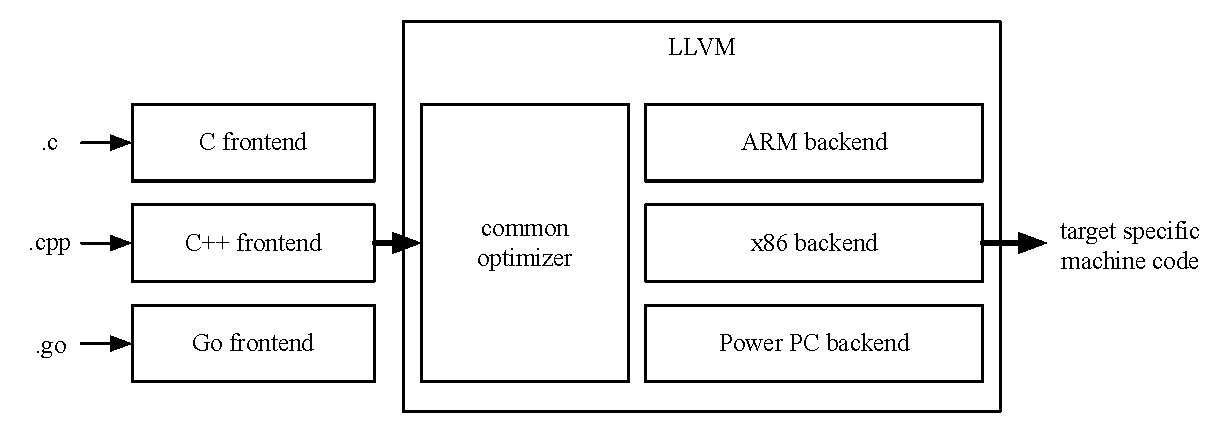
\includegraphics[width=10cm]{./figs/llvm}
\label{fig:llvm}
\caption{LLVM}
\end{figure}

我们依托LLVM构建NVM,如图\ref{fig:nvm}所示。首先,我们提供区块链底层API库;然后,利用LLVM链接我们提供的底层库,完成核心协议和智能合约代码的编译、优化以及跨平台适配;最后,让这些代码通过LLVM的ExecutionEngine运行在NVM提供的安全的沙箱环境中。

\begin{figure}[h]
\centering
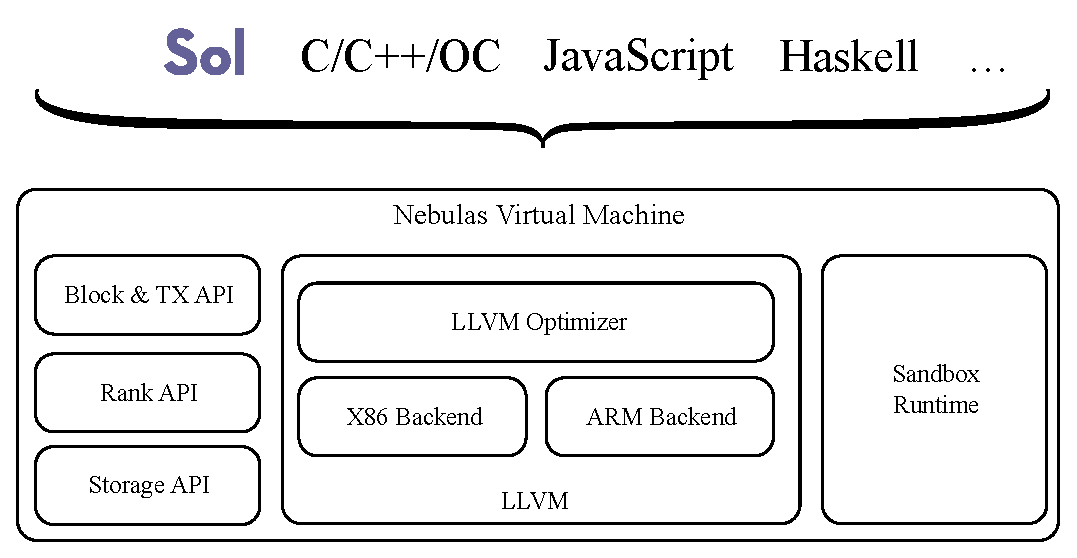
\includegraphics[width=10cm]{./figs/nvm}
\caption{星云链虚拟机}
\label{fig:nvm}
\end{figure}

NVM是星云原力的重要基石。新的协议代码或智能合约发布时,NVM中LLVM编译器模块完成新代码的编译得到NVM IR(Intermedia Representation),然后发布到链上,链上确认后新代码将由LLVM先做中间语言优化,然后进入沙箱取代旧代码执行,过程如图\ref{fig:nvm-process}所示。 \\

\begin{figure}[h]
\centering
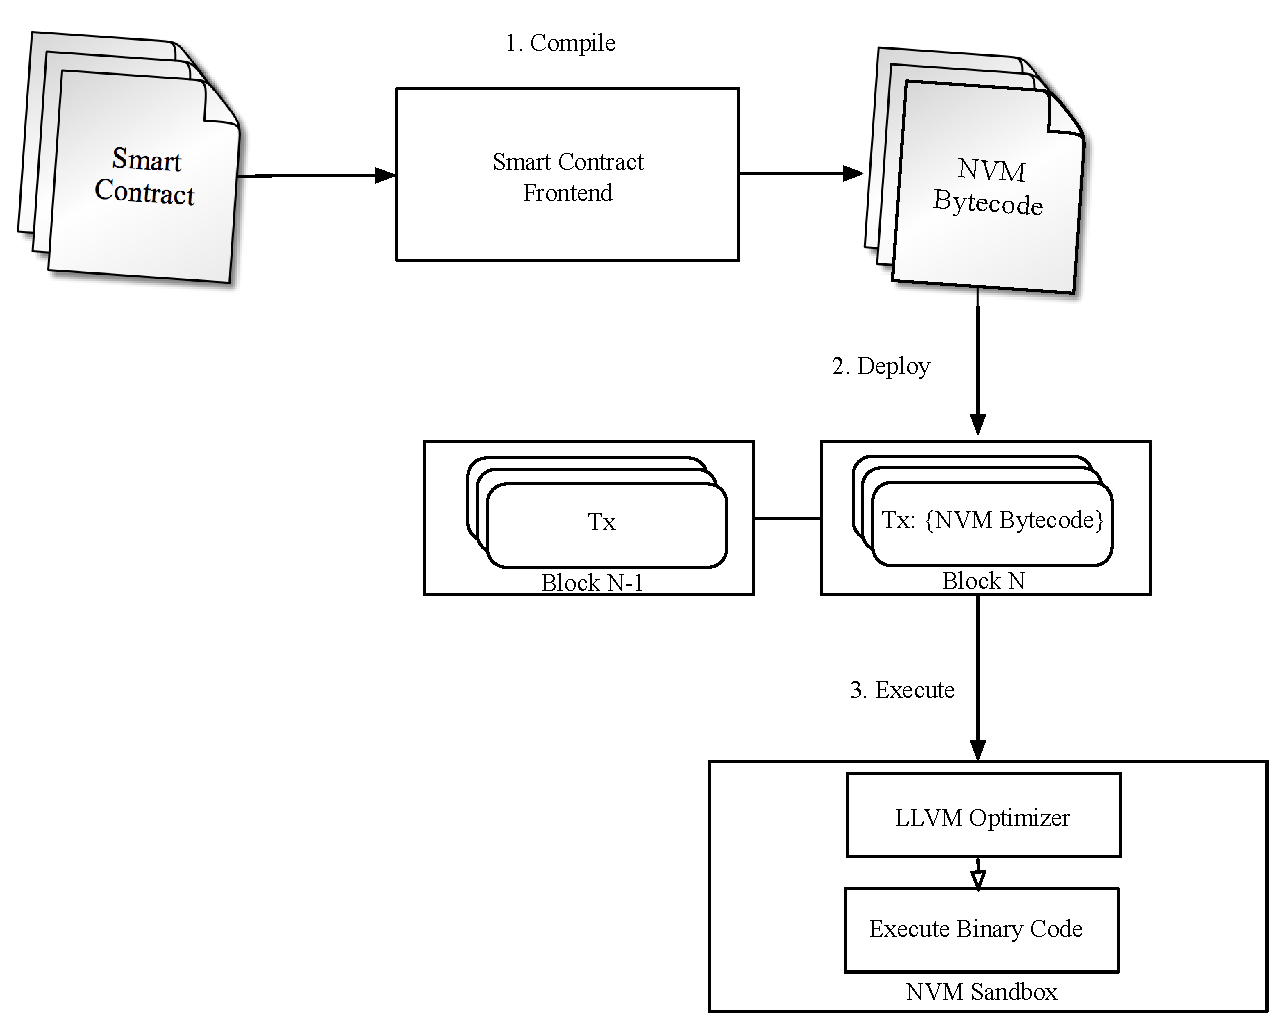
\includegraphics[width=10cm]{./figs/nvm-process}
\caption{星云链虚拟机运行机制}
\label{fig:nvm-process}
\end{figure}

除此之外,NVM还赋予了我们为上层应用构建更加丰富的前端的能力,如以太坊智能合约所使用的Solidity,语义更加灵活的Javascript,甚至可以为不同的领域的智能合约提供定制的高级语言,比如面向金融行业的DSL(领域专有语言)。 这类高级语言面向行业、场景高度定制,使得它们更容易被形式化验证,能进一步提高代码健壮性和安全性,更有利于星云链开发者开发出更丰富的智能合约及应用。
